\subsection{Sprint 3: 19.03 \textendash 01.04.2026}\label{subsec:sprint-3}

\subsubsection{Sprint Planning 3: 26.03.2026}\label{subsubsec:sprint-planning-3}

Because we got some important input regarding variant decision for \gls{AI}-integration, framework comparison, and configuration management~\ref{tab:meeting-notes-checkpoint-3} which led to additional work.
As consequence of this, we decided to shorten the third sprint to one week, which is reflected in the following table~\ref{tab:sprint-planning-3} and postponed the sprint planning from the 19.03 to the 26.03.
To account for the delayed start in the overall planning we adjusted t as shown in the ~\ref{fig:roadmap-sprint-planning-3}.

\begin{table}[H]
    \centering
    \begin{tabularx}{\textwidth}{l l X}
		\toprule
        \textbf{Week} & \textbf{Responsible} & \textbf{Task} \\
        \midrule
        Week 1 & Frank & Reproducible Test Environment implementation \\
        Week 1 & Lukas & \gls{NSAK} Scenario: \gls{AI} Scenarios (first part) \\
        \bottomrule
    \end{tabularx}
    \caption{Sprint Planning 3}
    \label{tab:sprint-planning-3}
\end{table}

\begin{figure}
    \centering
    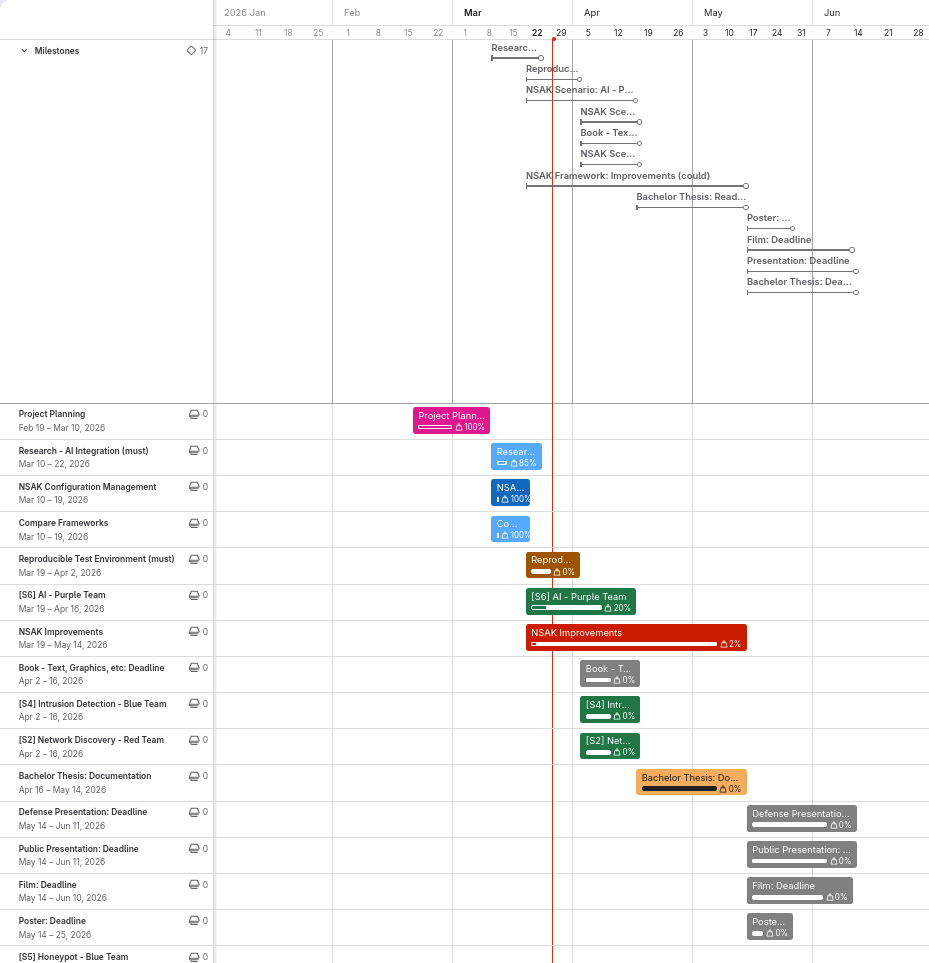
\includegraphics[width=1.0\linewidth]{../assets/screenshots/project_management/sprint_3/roadmap_sprint_planning_3}
    \caption{Roadmap Sprint Planning 3}
    \label{fig:roadmap-sprint-planning-3}
\end{figure}

\subsubsection{Sprint Review 3: 02.04.2026}\label{subsubsec:sprint-review-3}

\subsubsection{Sprint Retro 3: 02.04.2026}\label{subsubsec:sprint-retro-3}
\begin{figure}
	\centering
	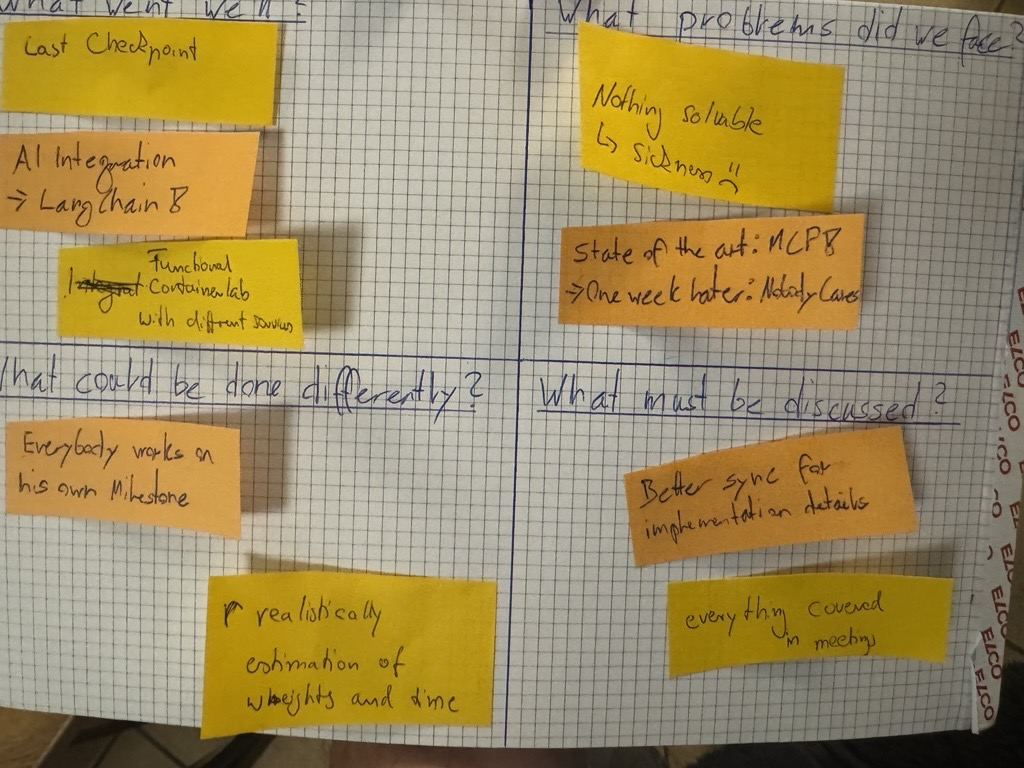
\includegraphics[width=0.7\linewidth]{../assets/screenshots/project_management/sprint_3/retro-sprint3}
	\caption{Retro Sprint 3}
	\label{fig:retro-sprint3}
\end{figure}

The Key Take Away of ~\ref{fig:retro-sprint3} are to estimate the milestones more realistically. We spend a lot of time with documentation which hinders the development. The upside of our continuous approach is a natural growing thesis which helps in the long run.
Overall, we are quite happy with the outcome of sprint 3.
